\section{Experiments}\label{m:sec:experiments}

Everything reported here is produced from fixed seeds by scripts that are supplied, with their recorded outputs, as ancillary files of our paper~\cite{polsonsokolov2026manifold} and described in Appendix~\ref{app:code}. The generator \texttt{make\_experiments\_tex.py} wrote the experiments section of that paper, tables included, directly from the resulting \texttt{json}, so every measured number in the tables and in the figure comes from a recorded run rather than being transcribed by hand. The setting is the heat equation of Section~\ref{m:sec:heat} on $\Omega=[0,1]$ with $\nu=0.01$, $T=1$, the fixed prior of that section with $\alpha=3$, and the conjugate Gaussian posterior available in closed form, so that the exact posterior is known and every approximation can be measured against it rather than against another approximation.

\subsection{The finite $N$ check, in the regime where the data speak}\label{m:sec:expfinite}

Table~\ref{m:tab:diag} reports the diagnosis. The first row is the uncalibrated setting of panel (a) of Figure~\ref{m:fig:heatgbc}, $\rho=1$ and $N=2000$: no mode has data precision exceeding prior precision. The agreement with the Bernstein von Mises scale there, $1.43\times10^{-4}$, is therefore not a validation of anything: both sides of the comparison are the prior, and a diagnostic that compares the prior with itself is vacuous whatever number it returns.

Two things are wrong at once and they have to be separated. The first is the scale of the prior, which $\rho$ fixes: calibrating $\rho$ so that the prior standard deviation at $|k|=1$ matches the initial condition there gives $\rho=124.0$, moves $k_{\rm eff}$ from $0$ to 2, covers every informed mode, and brings the relative $L^2$ error to $0.257$. The second is the shape: the initial condition $\theta_{0,k}=(1+k^2)^{-1}\mathrm{sign}(\sin k)$ decays like $k^{-2}$ whereas a draw from the fixed prior with $\alpha=3$ decays like $k^{-3}$, so after calibration the worst mode is still $39.9$ prior standard deviations out. That tail is invisible while $k_{\rm eff}$ is small and becomes visible as $N$ grows: the informed modes covered go from 2 of 2 at $N=2\times10^3$ to 3 of 5 at $N=1.3\times10^6$, with the worst standardized error over informed modes rising to $7.91$. Nothing is wrong with the posterior; the prior is wrong about the truth, and more data is what reveals it.

The last three rows replace the fixed $\theta_0$ by a draw from the prior itself, the only setting in which nominal coverage is the right thing to expect. Relative $L^2$ error stays near one at the smaller two, which is not a failure: this draw is small, with norm $0.0208$ against a prior root mean square norm of $0.50$, and the posterior standard deviations of its informed modes are of the same size ($0.027$ and $0.034$ at $N=2\times10^3$), so the error of the posterior mean is of the size of the signal itself and a ratio above one can occur while every informed mode stays within $2.2$ posterior standard deviations. Section~\ref{m:sec:resolution} says how many modes the data can resolve.

\begin{table}[t]\centering\footnotesize\setlength{\tabcolsep}{3pt}
\caption{The finite $N$ check for the heat equation. $k_{\rm eff}$ is the number of modes with $N\iota_k\ge\rho^{-2}\lambda_k^\alpha$; ``truth/prior sd'' is $\max_k|\theta_{0,k}|/\sigma_{0,k}$, a measure of how atypical the truth is under the prior; the coverage columns count the modes whose truth lies within two posterior standard deviations, over the informed modes and over all twenty; with $k_{\rm eff}$ this small these are counts and not estimates of a coverage probability, for which see the replicate study of Section~\ref{m:sec:expstudy}; $|z|_{\max}$ is the largest standardized error over informed modes; and the last column is the largest relative discrepancy, over all twenty modes, between the exact posterior standard deviation and the Bernstein von Mises (BvM) scale with the prior precision added, $(N\iota_k+\sigma_{0,k}^{-2})^{-1/2}$. The truth of the last block is a fixed draw from the prior that is typical in each coordinate but small in norm.}\label{m:tab:diag}
\begin{tabular}{rrrrrrrrr}
\toprule
$N$ & $\rho$ & $k_{\rm eff}$ & \shortstack[r]{truth/\\prior sd} & \shortstack[r]{cov.\\inf.} & \shortstack[r]{cov.\\all} & $|z|_{\max}$ & \shortstack[r]{rel.\\$L^2$} & \shortstack[r]{BvM\\rel.}\\
\midrule
\multicolumn{9}{@{}l}{Uncalibrated prior}\\
$2\times10^3$ & 1 & 0 & 4948.6 & n/a & 0 of 20 & n/a & 0.982 & $1.43\times10^{-4}$ \\
\addlinespace
\multicolumn{9}{@{}l}{Calibrated $\rho$}\\
$2\times10^3$ & 124 & 2 & 39.9 & 2 of 2 & 2 of 20 & 1.96 & 0.257 & $6.05\times10^{-3}$ \\
$5\times10^4$ & 124 & 3 & 39.9 & 3 of 3 & 3 of 20 & 0.92 & 0.144 & $1.60\times10^{-3}$ \\
$1.3\times10^6$ & 124 & 5 & 39.9 & 3 of 5 & 3 of 20 & 7.91 & 0.081 & $7.77\times10^{-4}$ \\
\addlinespace
\multicolumn{9}{@{}l}{Fixed draw from the prior}\\
$2\times10^3$ & 124 & 2 & 1.9 & 2 of 2 & 20 of 20 & 0.59 & 1.007 & $6.05\times10^{-3}$ \\
$5\times10^4$ & 124 & 3 & 1.9 & 2 of 3 & 19 of 20 & 2.18 & 1.270 & $1.60\times10^{-3}$ \\
$1.3\times10^6$ & 124 & 5 & 1.9 & 5 of 5 & 20 of 20 & 1.54 & 0.250 & $7.77\times10^{-4}$ \\
\bottomrule
\end{tabular}
\end{table}

\subsection{Cost and accuracy against the alternatives}\label{m:sec:expcost}

Table~\ref{m:tab:cost} reports what one analysis costs. Unless a variant is named, GBC in this table and in the rest of this section is Algorithm~\ref{m:alg:loc} with $c=2$ and the identity head, applied to the regularized summary of Remark~\ref{m:rem:reg}. The units are forward or adjoint solves of the linearized equation, which is the currency in which data assimilation is priced, together with wall clock for the methods actually run here. The two comparators are the Laplace approximation at the posterior mode and the preconditioned Crank Nicolson sampler (pCN), in the form given by Cotter and coauthors~\cite{cotter2013}.

\begin{table}[t]\centering\footnotesize\setlength{\tabcolsep}{4pt}
\caption{Cost and accuracy for one analysis of the heat equation, $N=50000$, $|k|\le8$, single core. Errors are the maximum over the retained modes, in units of the exact posterior standard deviation (psd). ``Amortized'' records whether a second data set can be analyzed without repeating the cost. $\dagger$: analytic, not measured. In this linear Gaussian model both the Laplace approximation at the posterior mode and the GBC generator have the exact posterior mean, by Proposition~\ref{m:prop:linsuff}, so their mean error is exactly zero at every budget. The standard deviation ratio, the median over the retained modes of the reported posterior standard deviation divided by the exact one, is the column that carries information here. Neither the $8000$ solves of GBC, a forward and an adjoint solve for each of its $M=4000$ simulations, nor the $2$ of Laplace, one forward and one adjoint solve, include forming the Gauss Newton covariance $(\Phi^\top\Phi+\Sigma_0^{-1})^{-1}$, which is the covariance of the Laplace row and which GBC's localized proposal and summary also use. It is formed once in either method and takes one further linearized solve per retained mode, $8$ here; the Laplace time is that of forming it from $\Phi$, and the GBC time, which covers the simulations, the fit and the $4000$ draws, leaves it out.}\label{m:tab:cost}
\begin{tabular}{lrrrrl}
\toprule
Method & Solves & Time (s) & \shortstack[r]{Max err.\\(psd)} & \shortstack[r]{sd\\ratio} & Amortized\\
\midrule
GBC, Algorithm~\ref{m:alg:loc}, $c=2$ & 8000 & 2.91 & $0^{\dagger}$ & 1.003 & amortized \\
Laplace at $\hat S_N$ & 2 & 0.0003 & $0^{\dagger}$ & $1^{\dagger}$ & no \\
pCN, $2\times10^{5}$ iterations & 200000 & 86.5 & 0.325 & 0.947 & no \\
\bottomrule
\end{tabular}
\end{table}

Three readings. First, GBC is not more accurate than Laplace and cannot be: by Definition~\ref{m:def:gen} its generator is a Monte Carlo estimate of the Laplace approximation, so its mean is that approximation's mean exactly, and the $0.016$ posterior standard deviations one reads off the worst of its $4000$ output draws is the sampling error of those draws, not an error of the method. What it buys over Laplace is that the forward map is reached only by simulation and that no Hessian is evaluated at the training draws: the one Gauss Newton covariance of Algorithm~\ref{m:alg:loc} is formed once, at the preliminary estimate (Remark~\ref{m:rem:whichcov}). Second, pCN is included to exhibit the Monte Carlo rate the two methods share, not as a tuned competitor: in this conjugate model the exact posterior is a known Gaussian that can be sampled directly and a whitened or Gibbs sampler would mix in one step, so the comparison is not in GBC's favor on a single data set: $200000$ iterations and a tuned acceptance rate of 0.246 at $\beta=0.0491$ deliver a minimum effective sample size of 16 across the retained modes, which is why its worst mode error is larger than GBC's and is Monte Carlo noise rather than bias: its posterior standard deviation ratio is 0.947. Given enough iterations pCN is exact and GBC is not. Third, the cost that matters operationally is the ratio to a 4DVar minimization. Neither 4DVar nor an ensemble Kalman filter (EnKF) is run here: a 4DVar minimization returns a point estimate, and an ensemble filter returns an ensemble that is a posterior sample only for a linear forward map and a large ensemble, so no error in these units is reported for either. Both do have conventional solve counts: 20 for a Gauss Newton 4DVar at ten inner iterations of one forward and one adjoint solve, and one solve per ensemble member for an ensemble filter. Against those conventions one GBC analysis is 400 4DVar equivalents at $M=4000$ and 80 times a 100 member EnKF. Those are the numbers Section~\ref{m:sec:related} refers to, and they are the price of amortization: the 4000 simulations are spent once, and every subsequent data set is a forward pass.

\subsection{Error against cost, and coverage over replicates}\label{m:sec:expstudy}

The error against cost and the coverage over replicates are both studied at $N=50000$ with $D=8$ modes retained, of which $k_{\rm eff}=3$ are data dominated, and at the calibrated $\rho=124$ of Section~\ref{m:sec:expfinite}. A single realization cannot separate a miscalibrated posterior from an unlucky draw, so calibration is checked over replicates, on three truth arms. The result, set out in Section~\ref{m:sec:covstudy} and shown for the arm drawn from the prior in the lower panel of Figure~\ref{m:fig:cost}, is that GBC reproduces whatever the exact posterior does, on every arm, under a paired McNemar test that takes the replicate as its unit.

In the linear Gaussian model of Section~\ref{m:sec:heat} Proposition~\ref{m:prop:linsuff} gives the mean map in closed form, so GBC's posterior mean is exact at every budget and only the $D\times D$ covariance is estimated from the $M$ simulations. Scoring the mean therefore measures nothing about the method: over 40 replicates and 8 budgets, 320 measurements in all, its error is exactly zero (Remark~\ref{m:rem:artifact}).

\begin{remark}[Why a finite draw mean error is not an approximation floor]\label{m:rem:artifact}
Scoring GBC's posterior mean against the exact one in this model measures a quantity whose value is exactly zero, so any nonzero reading is the sampling noise of however many output draws were taken. Holding that count fixed at 4000 while the simulation budget sweeps a factor of 128 returns 0.023 to 0.044 posterior standard deviations with a fitted slope against the budget of $-0.029$, flat. That flatness is not an approximation floor of the plug in generator. The quantity decays in the number of output draws, not in $M$, so no simulation budget can move it and there is nothing there to converge. A Gaussian head does carry a genuine approximation error wherever the posterior is not Gaussian, but a linear Gaussian benchmark is precisely the case in which that error vanishes identically, so this diagnostic cannot measure it at any budget. Any study of a Gaussian head generator that scores the mean on a conjugate benchmark meets the same trap.
\end{remark}

What the simulations buy is the covariance, and scored analytically it converges at the Monte Carlo rate with no floor. Across the 3 generator variants and both covariance metrics the fitted slope of $\log$ error against $\log$ solves lies between $-0.521$ and $-0.495$ against a nominal $-1/2$, with replicate standard error 0.009; raising $M$ from 250 to 32000 cuts the error on the standard deviations from 0.081 to 0.0071. The learned mean variant, which ignores Proposition~\ref{m:prop:linsuff} and regresses $\theta$ on the summary from the same simulations, does carry a mean error, converging at $-0.514$ to 0.030 at the largest budget: that gap is what the affine structure is worth. pCN has no floor either. Its error on the standard deviations falls from 0.577 to 0.053 as the budget grows from $5.0\times10^{3}$ to $1.3\times10^{6}$ solves. Its rate has to be read with the mixing in view: the minimum effective sample size over the retained modes is 4 at the smallest budget and 131 only at the largest, so the smallest budgets measure how far the chain has failed to move rather than a Monte Carlo error. Fitting all 5 gives $-0.423$; fitting the 3 budgets with an effective sample size above 7 gives $-0.507$, which is the Monte Carlo rate and is what we use below.

So both methods converge at essentially the same rate, $-0.521$ for GBC against $-0.507$ for pCN on the standard deviations. The advantage is therefore a constant factor rather than a widening gap, and it can be read off without extrapolating either curve beyond where it was measured. Over the band of accuracy both methods reached, 0.081 down to 0.053 posterior standard deviations, pCN needs between 1154 and 1181 times as many solves as GBC to match it on the standard deviations, and between 366 and 510 times as many on the full covariance, over the band 0.140 down to 0.063 of relative error in Frobenius norm that both reached on that metric. Solves, not seconds, are the currency: wall clocks depend on the machine and its load (Appendix~\ref{app:code} records a rerun on a busier machine). The choice between the two methods turns on how many solves an application can afford.

\begin{figure}[tp]\centering
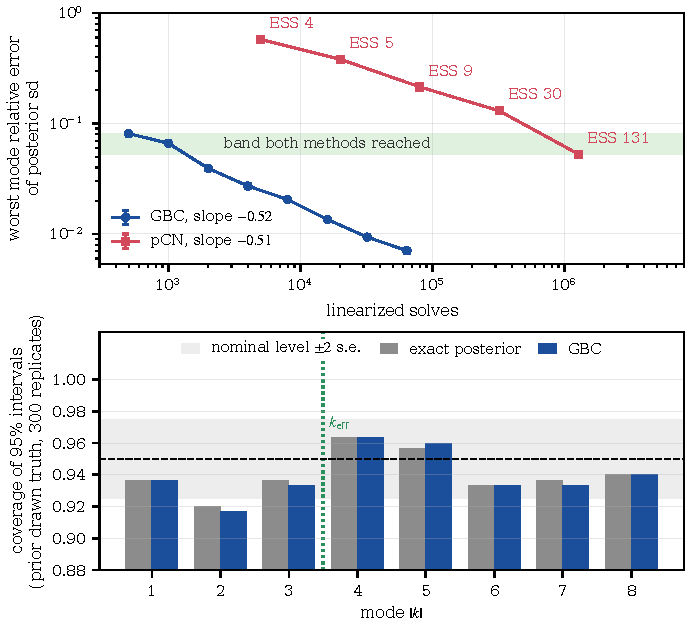
\includegraphics[width=0.94\textwidth]{mf_cost}
\caption{Upper panel: error against the number of linearized solves, on the metric the simulations actually control. GBC's posterior mean is exact at every budget in this model (Proposition~\ref{m:prop:linsuff}), so what is plotted is the error of the estimated posterior standard deviations, in units of the exact ones, taken as the largest over the retained modes and averaged over 40 replicates, for GBC at $M=250$ to $32000$ and for pCN at $5.0\times10^{3}$ to $1.3\times10^{6}$ iterations; the bars are one standard error over replicates, and the labels give the minimum over modes of the effective sample size (ESS) of the pCN chain, averaged over replicates. Both follow the Monte Carlo rate and neither has a floor. The shaded band is the range of accuracy both reached. Lower panel: coverage of nominal $95\%$ credible intervals by mode, over 300 replicates of the arm in which $\theta_0$ is drawn from the prior, for the exact posterior and for GBC; the shaded band is the nominal level plus or minus two binomial standard errors, and the dotted line marks $k_{\rm eff}$, beyond which the intervals are the prior's. Over the 2400 (replicate, mode) pairs of that arm the two disagree on 5 pairs against 3, each in a different replicate, a coverage difference of 0.0008 (Table~\ref{m:tab:cover}).}\label{m:fig:cost}
\end{figure}

\subsection{Coverage over replicates, in full}\label{m:sec:covstudy}

Table~\ref{m:tab:cover} has the numbers in full. Hypothesis (G1) of Assumption~\ref{m:ass:G} is stated in $P^\N_{\theta_0}$ probability at a \emph{fixed} $\theta_0$, and redrawing $\theta_0$ from the prior at every replicate makes the exact posterior's coverage nominal by construction, so under that design alone the comparison cannot fail informatively. The three arms are therefore $\theta_0$ redrawn from the prior, a fixed typical draw, and a fixed rough truth $\theta_{0,k}=(1+k^2)^{-1}\mathrm{sign}(\sin k)$, which the prior charges only in its tail. With $M=4000$ simulations, each arm has 300 replicates.

\begin{table}[t]\centering\footnotesize\setlength{\tabcolsep}{4pt}
\caption{Coverage of nominal $95\%$ credible intervals over 300 replicates per arm, by truth arm. ``All'' is over the $D=8$ retained modes, ``informed'' over the $k_{\rm eff}=3$ modes in which data precision exceeds prior precision. $b/c$ are the discordant counts, the (replicate, mode) pairs that the exact posterior covers and GBC misses and the reverse, out of $2400$. With $x_r$ the number of modes of replicate $r$ that the exact posterior covers and GBC misses minus the number of the reverse, $z=\sum_rx_r/(\sum_rx_r^2)^{1/2}$ is the clustered McNemar statistic of Durkalski and coauthors~\cite{durkalski2003}, and $p$ is the exact two sided $p$ value of the sign flip test, which gives each nonzero $x_r$ an independent random sign, as it has when the two methods are exchangeable within a replicate. The rough arm is misspecified by construction: its truth decays like $k^{-2}$, whereas a draw from the prior of smoothness $\alpha=3$ used here decays like $k^{-3}$, so both methods undercover, and identically; a draw from a prior with $\alpha>12$, the smoothness that Konen and Nickl~\cite{konennickl2026} require for the Navier Stokes problem, decays faster still. That the exact posterior undercovers too is the point of including the arm.}\label{m:tab:cover}
\begin{tabular}{>{\raggedright\arraybackslash}p{1.5in}ccccccc}
\toprule
& \multicolumn{2}{c}{All modes} & \multicolumn{2}{c}{Informed modes} & & & \\
\cmidrule(lr){2-3}\cmidrule(lr){4-5}
Truth arm & exact & GBC & exact & GBC & $b/c$ & $z$ & $p$\\
\midrule
$\theta_0\sim\Pi$, redrawn each replicate & 0.940 & 0.940 & 0.931 & 0.929 & $5$/$3$ & $0.71$ & $0.73$\\
fixed typical draw & 0.843 & 0.845 & 0.914 & 0.919 & $2$/$6$ & $-1.63$ & $0.22$\\
fixed rough truth & 0.251 & 0.251 & 0.670 & 0.670 & $1$/$1$ & $0.00$ & $1.00$\\
\bottomrule
\end{tabular}
\end{table}

Two things separate here. First, the exact posterior does not have frequentist coverage at a fixed truth and is not required to: its coverage over all $D$ retained modes falls from 0.940 on the prior drawn arm to 0.843 at the fixed typical draw and 0.251 at the rough one. That is the shrinkage of the posterior mean, milder on the informed modes, which averaging over the prior hides; as $N\to\infty$ each mode is covered at the nominal rate, with $D=8$ as here and, by Proposition~\ref{m:prop:regfixed}, with $D$ growing, but slowly at the rough truth.

Second, and this is the claim we make, GBC reproduces whatever the exact posterior does. Both methods are scored on the same replicate and the same mode, so the yardstick is a paired comparison, McNemar's, and not the binomial standard error of a single coverage estimate. The pairs of one replicate are not independent, since its eight modes are computed from the same data, so the comparison is made over the 300 independent replicates: the statistic of Table~\ref{m:tab:cover} is $z=\sum_rx_r/(\sum_rx_r^2)^{1/2}$. Where no replicate holds more than one discordant pair, as on the prior drawn and the rough arm, that statistic and its exact test are McNemar's own; on the typical arm one replicate holds one discordant pair of each kind. The standard error that the test gives the difference of the coverages, $(\sum_rx_r^2)^{1/2}/2400$, is between 11 and 21 times smaller than the binomial standard error at the nominal level of the coverage of a single mode over the 300 replicates, and between 5 and 7 times smaller than the standard error of the difference of the coverages over all modes of two methods run on independent data, so the test is several times more sensitive than the comparison it replaces. GBC survives it on every arm. The largest discrepancy across the three is 1.63 standard errors, on the typical arm, with exact $p$ value 0.22, and the largest difference in coverage over all modes is 0.0017; on the rough arm, where the exact posterior covers barely a quarter of the time, the two disagree on $2$ of $2400$ pairs, one each way.

The calibration claim is therefore relative rather than absolute: GBC reproduces the posterior it targets, including where that posterior is badly miscalibrated as a frequentist procedure. Coverage at a fixed truth is a property of the prior and the model rather than of the computation. One qualification: both arms of the comparison use the same summary, the adjoint statistic of Lemma~\ref{m:lem:adjoint}, and, by Proposition~\ref{m:prop:linsuff}, the same closed form posterior mean, so what differs between them is the covariance, exact in one case and estimated from the $M$ simulations in the other. The agreement is evidence that the estimated covariance is right, and is not a test of the summary or of the centering.
